%Dokumentklasse

%draft als optionohne bilder für bessere performance
%\documentclass[a4paper,12pt,draft]{scrreprt}

%normal mit Bildern
\documentclass[a4paper,12pt]{scrreprt}

\usepackage[left= 3cm,right = 3cm, bottom = 3cm,top = 3cm]{geometry}
%\usepackage[onehalfspacing]{setspace}

% ============= Packages =============

% Dokumentinformationen
\usepackage[
	pdftitle={Praktikum - Umwelttechnik},
	pdfsubject={},
	pdfauthor={Roman-Luca Zank},
	pdfkeywords={},	
	%Links nicht einrahmen
	hidelinks
]{hyperref}

%nur Text zum prüfen des Umfangs

% Standard Packages
\usepackage[utf8]{inputenc}
\usepackage{cancel}
\usepackage[ngerman]{babel}
\usepackage[T1]{fontenc}
\usepackage{graphicx}
\graphicspath{{img/}}
\usepackage{fancyhdr}
\usepackage{lmodern}
\usepackage{color}
\usepackage{placeins}
\usepackage{booktabs}
\usepackage{caption}
\usepackage[list=true]{subcaption}
\usepackage{mhchem}

%Einheitenpackage
\usepackage{siunitx}  
\sisetup{	locale = DE, 
			per-mode=fraction,
			inter-unit-product=\ensuremath{\cdot},
			detect-weight = true,
			quotient-mode=fraction
		}
%neue Einheiten definieren
\DeclareSIUnit\xyz{xyz}	
\DeclareSIUnit\d{d}	
\DeclareSIUnit\ppm{ppm}		

%Automatisch cdot statt *
\DeclareMathSymbol{*}{\mathbin}{symbols}{"01}

%d klein in Mathemodus
\newcommand*\diff{\mathop{}\!\mathrm{d}}
\newcommand*\Diff[1]{\mathop{}\!\mathrm{d^#1}}



%\setcounter{lofdepth}{2}      %für subfigures in list of figures

%Tabelle
\usepackage{tabularx}
\usepackage{tabulary}

%%Verzeichnispackages
%\usepackage{natbib}

%\usepackage{hyperref}
%\newcites{

% zusätzliche Schriftzeichen der American Mathematical Society
\usepackage{amsfonts}
\usepackage{amsmath}

%Abkürzungsverzeichnis
\usepackage{acronym}

%kein Abstand bei neuem Kapitel vom Seitenanfang
%\vspace*{2.3\baselineskip} = ORIGINAL
\renewcommand*{\chapterheadstartvskip}{\vspace*{.0\baselineskip}}

%nicht einrücken nach Absatz
\setlength{\parindent}{0pt}

% ============= Kopf- und Fußzeile =============
\pagestyle{fancy}
%
\lhead{}
\chead{}
\rhead{}%\slshape }%\leftmark}
%%
\lfoot{}
\cfoot{}
\rfoot{\pagemark}
%%
\renewcommand{\headrulewidth}{0pt}
\renewcommand{\footrulewidth}{0pt}
\renewcommand{\chapterpagestyle}{fancy}

% ============= Package Einstellungen & Sonstiges ============= 
%Besondere Trennungen
%\hyphenation{De-zi-mal-tren-nung}
\usepackage[none]{hyphenat}
\hyphenpenalty=5000
\tolerance=5000
\providecommand\phantomsection{}

\usepackage{mathtools}

% ============= Dokumentbeginn =============

\begin{document}
%Seiten ohne Kopf- und Fußzeile sowie Seitenzahl
\pagestyle{empty}

%\begin{center}
\begin{tabular}{p{\textwidth}}


\begin{center}

\includegraphics[scale=0.75]{img/logos.jpg}\\
\end{center}


\\

\begin{center}
\LARGE{\textsc{
Protokoll \\
Umwelttechnik\\
}}
\end{center}

\\

%\begin{center}
%\large{Fakultät für Muster und Beispiele \\
%der Hochschule Musterhausen \\}
%\end{center}
%
%\\

\begin{center}
\textbf{\Large{V4 - Bodencharakterisierung}}
\end{center}

\begin{center}
	\large{Gruppe 1.2 (BCUT3)}
\end{center}


\\
%\begin{center}
%zur Erlangung des akademischen Grades\\
%Bachelor of Engineering
%\end{center}


%\begin{center}
%vorgelegt von
%\end{center}

\begin{center}
\Large{\textbf{Teilnehmer:}} \\ 
\end{center}
\begin{center}
\large{Willy Messerschmidt \\
		Roman-Luca Zank} \\
\end{center}


\\

\begin{center}
\begin{tabular}{lll}
\large{\textbf{Protokollführer:}} & & \large{Roman oder Willy} \\
& & email@stud.hs-merseburg.de\\
&&\\
\large{\textbf{Datum der Versuchsdurchführung:}}&& \large{12.12.2019}\\
&&\\
\large{\textbf{Abgabedatum:}}&& \large{12.12.2019}
\end{tabular}
\end{center}

\\ \\ \\ \\ \\ \\ \\ 
\large{Merseburg den \today}

\end{tabular}
\end{center}


%\include{14_danksagungen}

%\include{15_zusammenfassung}

% Beendet eine Seite und erzwingt auf den nachfolgenden Seiten die Ausgabe aller Gleitobjekte (z.B. Abbildungen), die bislang definiert, aber noch nicht ausgegeben wurden. Dieser Befehl fügt, falls nötig, eine leere Seite ein, sodaß die nächste Seite nach den Gleitobjekten eine ungerade Seitennummer hat. 
\cleardoubleoddpage

% Pagestyle für Titelblatt leer
\pagestyle{empty}

%Seite zählen ab
\setcounter{page}{0}

%Titelblatt
%\begin{center}
\begin{tabular}{p{\textwidth}}


\begin{center}

\includegraphics[scale=0.75]{img/logos.jpg}\\
\end{center}


\\

\begin{center}
\LARGE{\textsc{
Protokoll \\
Umwelttechnik\\
}}
\end{center}

\\

%\begin{center}
%\large{Fakultät für Muster und Beispiele \\
%der Hochschule Musterhausen \\}
%\end{center}
%
%\\

\begin{center}
\textbf{\Large{V4 - Bodencharakterisierung}}
\end{center}

\begin{center}
	\large{Gruppe 1.2 (BCUT3)}
\end{center}


\\
%\begin{center}
%zur Erlangung des akademischen Grades\\
%Bachelor of Engineering
%\end{center}


%\begin{center}
%vorgelegt von
%\end{center}

\begin{center}
\Large{\textbf{Teilnehmer:}} \\ 
\end{center}
\begin{center}
\large{Willy Messerschmidt \\
		Roman-Luca Zank} \\
\end{center}


\\

\begin{center}
\begin{tabular}{lll}
\large{\textbf{Protokollführer:}} & & \large{Roman oder Willy} \\
& & email@stud.hs-merseburg.de\\
&&\\
\large{\textbf{Datum der Versuchsdurchführung:}}&& \large{12.12.2019}\\
&&\\
\large{\textbf{Abgabedatum:}}&& \large{12.12.2019}
\end{tabular}
\end{center}

\\ \\ \\ \\ \\ \\ \\ 
\large{Merseburg den \today}

\end{tabular}
\end{center}
 %Prokolle
\begin{center}
\begin{tabular}{p{\textwidth}}


\begin{center}

\includegraphics[scale=0.75]{img/logos.jpg}\\
\end{center}


\\

\begin{center}
\LARGE{\textsc{
Physikalische Chemie I\\
}}
\end{center}

%\begin{center}
%\large{Fakultät für Muster und Beispiele \\
%der Hochschule Musterhausen \\}
%\end{center}
%
%\\
 \\
 
\begin{center}
\textbf{\Large{Skriptaufzeichnungen}}
\end{center}

\begin{center}
	\large{im WiSe 2019}
\end{center}
 \\
%\begin{center}
%zur Erlangung des akademischen Grades\\
%Bachelor of Engineering
%\end{center}


\begin{center}
\large{vorgelegt von}
\end{center}
\\


\begin{center}
\Large{\textbf{Roman-Luca Zank}} \\
\end{center}

\begin{center}
3. Semester \\
Chemie- und Umwelttechnik \\
\end{center}


\begin{center}
\begin{tabular}{lll}
	\textbf{E-Mail:} & & romanzank@mail.de\\
	\textbf{Matrikelnummer:} & &25240\\
	\textbf{Adresse:} & &Platz der Bausoldaten 2, Zimmer 224\\
	\textbf{Ort:} & &06217 Merseburg\\
	&& \\
	\textbf{Prüfer:} & & Reinhold\\
\end{tabular}
\end{center}

\\ \\ \\ \\ \\
\large{Merseburg, \today}

\end{tabular}
\end{center}
 %Seminar-/Abschlussarbeit

% Pagestyle für Rest des Dokuments
\pagestyle{fancy}

%Inhaltsverzeichnis
\tableofcontents

%Inhalt

%%Verzeichnis aller Bilder
%\label{sec:bilder}
%\listoffigures
%\addcontentsline{toc}{chapter}{Abbildungsverzeichnis}

%Verzeichnis aller Tabellen
%\label{sec:tabellen}
%\listoftables
%\addcontentsline{toc}{chapter}{Tabellenverzeichnis}

%%Abkürzungsverzeichnis
%\setlength{\columnsep}{20pt}
%\twocolumn
%\addchap{Nomenklatur (fett)}
%\label{sec:abkurzung}
%\begin{acronym}
%	\acro{vbr} [\boldmath{$\dot{V}_{Br}$}] {Volumenstrom Brennstoff \\ (Erdgas)}
%	\acro{vml} [\boldmath{$\dot{V}_{L}$}] {Volumenstrom der Luft}
%	\acro{vwa} [\boldmath{$\dot{V}_{W\omega}$}] {Ausgangsvolumenstrom Wasser}
%	\\
%	\acro{mbr} [\boldmath{$\dot{m}_{Br}$}] {Massestrom Brennstoff \\ (Erdgas)}
%	\acro{ml}  [\boldmath{$\dot{m}_{L}$}] {Massenstrom Luft}
%	\acro{ma}  [\boldmath{$\dot{m}_{A}$}] {Massenstrom Abgas}
%	\acro{mwa} [\boldmath{$\dot{m}_{W\alpha}$}] {Eingangsmassenstrom Wasser}
%	\acro{mww} [\boldmath{$\dot{m}_{W\omega}$}] {Ausgangsmassenstrom Wasser}
%	\\
%	\acro{qbr} [\boldmath{$\dot{Q}_{Br}$}] {Wärmestrom Brennstoff \\ (Erdgas)}
%	\acro{qa}  [\boldmath{$\dot{Q}_{A}$}] {Wärmestrom Abgase}
%	\acro{qstr}[\boldmath{$\dot{Q}_{Str}$}] {Strahlungswärme}
%	\acro{qw}  [\boldmath{$\dot{Q}_{W}$}] {result. Wärmestrom Wasser}
%	\acro{qwe} [\boldmath{$\dot{Q}_{Weitere}$}] {Weitere Wärmeverluste}
%	\\
%	\acro{nbro} [\boldmath{$\dot{n}_{Br}$}] {Molstrom Brennstoff}
%	\acro{no2o} [\boldmath{$\dot{n}_{O_{2}}$}] {Molstrom Sauerstoff}
%	\\
%	\acro{wirkungE} [\boldmath{$\eta_{E}$}] {energetischer Wirkungsgrad}
%	\acro{wirkungF} [\boldmath{$\eta_{F}$}] {feuerungstechnischer\\ Wirkungsgrad}
%	\\
%	\acro{vT} [\boldmath{$\tau_{Vor}$}] {Heizvorlauftemperatur}
%	\acro{rT} [\boldmath{$\tau_{Rück}$}] {Heizrücklauftemperatur}
%	\acro{AT} [\boldmath{$\tau_{A}$}] {Abgastemperatur}
%	\acro{averlust} [\boldmath{$qA$}] {Abgasverlust}
%	\acro{co2}[\boldmath{$\%CO_{2}$}] {CO$_{2}$-Gehalt im Abgas}
%	\acro{o2} [\boldmath{$\%O_{2}$}] {O$_{2}$-Restgehalt im Abgas}
%	\\
%	\acro{heizbr} [\boldmath{$H_u$}$= 10,4 \frac{kWh}{m^3}$] {Heizwert \\ des Brennstoffes (Erdgas)}
%	\acro{dbr}[\boldmath{$\rho_{E}$}$= 0,7\frac{kg}{m^3}$] {Dichte \\ des Brennstoffes (Erdgas)}
%	\acro{dw} [\boldmath{$\rho_{W}$}$= 988\frac{kg}{m^3}$] {Dichte \\ des Heizfluides (Wasser)}
%	\acro{dl} [\boldmath{$\rho_{L}$}$= 1,2\frac{kg}{l}$] {Dichte der Luft}
%	\acro{cp} [\boldmath{$c_{pW}$}$= 4,1\frac{kJ}{kg*K}$] {spezifische \\ Wärmekapazität des Heizfluides (Wasser)}
%	\acro{nbr} [\boldmath{$M_{Br}= 16\frac{g}{mol}$}] {Molare Masse \\ des Brennstoffs}
%\end{acronym}
%\subsubsection{Aufrufen einer Abkürzung}
%\acs{rT}
%\begin{verbatim}
%\acs{Abkürzung}
%\end{verbatim}
%\onecolumn

\include{03_einfühurng}

\chapter{Thermodynamik}
\section{Grundbegriffe der Thermodynamik}
\textbf{Energie E}\\
= Fähigkeit eines Systems Arbeit zu verrichten
\begin{itemize}
	\item kinet. E = $\frac{1}{2}*m*v^2$
	\item elektr. E = $U/d$
	\item pot. E = $m*g*h$
	\item Wärmeenergie = $m*c_p+\Delta T$ , wenn $p=const.$
	\item Photonenenergie = $h*f$
\end{itemize}

\textbf{Arbeit W}
\begin{itemize}
	\item mech. Arbeit = $F*s$
	\item elektr. Arbeit = $P*t=I^2*R*t$
	\item Volumenarbeit = $-p*\text{d}V$
\end{itemize}

\textbf{Leistung P} = $\frac{W}{t}$\\ \\

\textbf{\underline{Arten von Systemen:}}
\begin{itemize}
	\item \textbf{offenes System}: Energie und Stoff
	\item  \textbf{geschlossenes System}: Energie
	\item  \textbf{abgeschlossenes System}: nichts ("`adiabat"') 
\end{itemize}

\section{Ideales Gasgesetz}
\textbf{Satz von Avogadro}: \\
$V=\text{Konstante}*n$ für $T,p = const.$\\

\textbf{Gesetz von Gay-Lussac}: \\
$V=\text{Konstante}*T$ für $n,p = const.$\\

\textbf{Boyle-Marriot'sche Gasgesetz}: \\
$p*V=const.$ für $n,T = const.$\\

\textbf{Ideales Gasgesetz}: \\
$\frac{p*V}{n*T}=R\rightarrow \boldsymbol{p*V=n*R*T} \rightarrow p*V_m=R*T\rightarrow p*V=m*R_{sp}*T$

\section{erster Hauptsatz der Thermodynamik}
\subsection{Größen des 1. HS}

\textbf{Arbeit d$W$}\\
= gerichtete Bewegung der Teilchen, z.B. Volumenarbeit $\rightarrow$ Prozessgröße\\

\textbf{Wärme $Q$}\\
= ungerichtete Bewegung der Teilchen (Rotation, Translation, Vibration) $\rightarrow$ Prozessgröße\\

\textbf{innere Energie $U$}\\
= entspricht der Gesamtenergie eines Systems, beschreibt als makroskopische Größe Gesamtheit des \underline{Energiespektrums} {\tiny{(Translation, opt. Anregung, Rotation,...)}} aller Teilchen/Moleküle im System \\ \\
= Zustandsgröße (spielt keine Rolle ob $E$ durch $W$ oder $Q$ zugeführt wurde)

\begin{center}
	"`je höher die innere Energie, desto höher besetzt sind auch die Energieniveaus im Energiespektrum der Teilchen bzw. deren Energiewerte"'
\end{center}

%Start
\begin{figure}[h!]
	\centering
	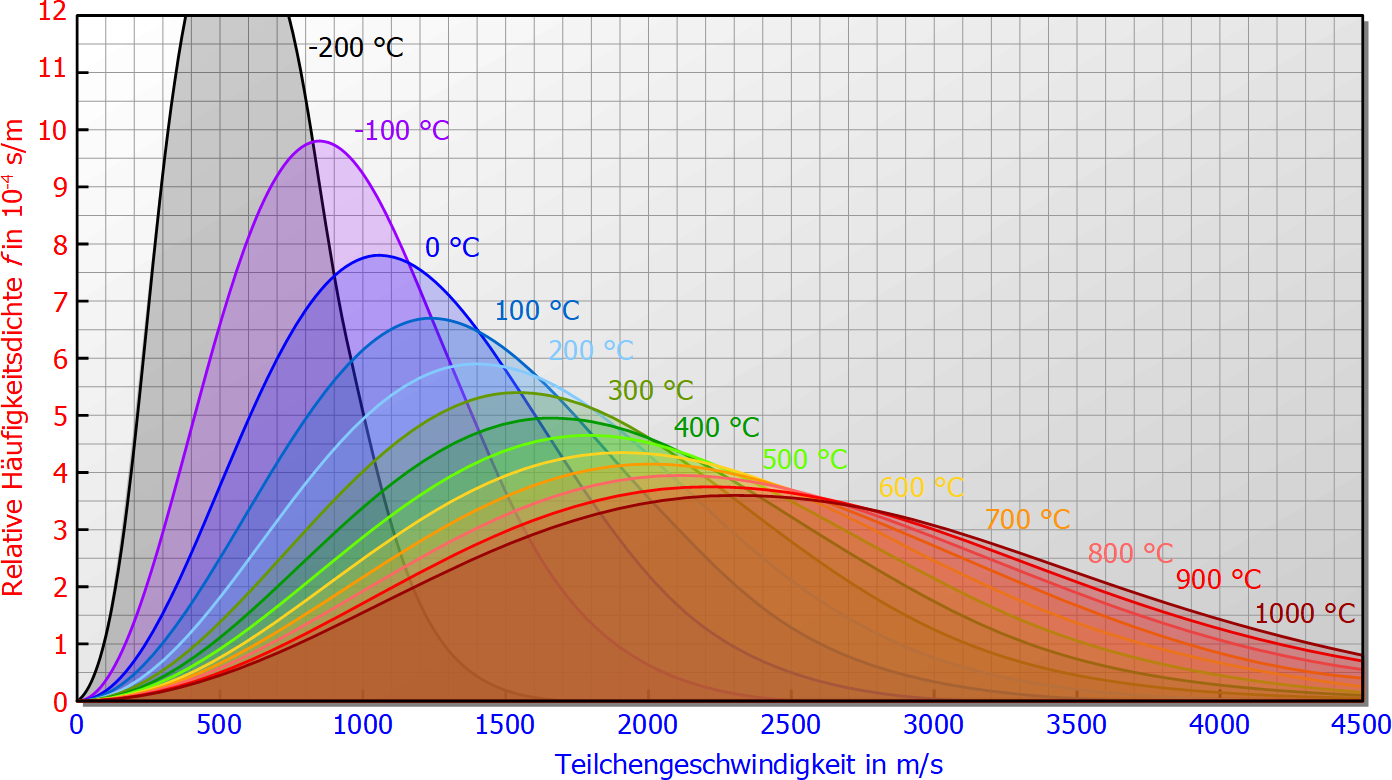
\includegraphics[width=0.75\textwidth]{img/boltzmann}
	\caption{Boltzmann-Verteilung}
\end{figure}
\FloatBarrier
%Ende

\newpage

\subsection{Allg. Beschreibung 1. HS Thermodynamik}
\begin{center}
	"`die innere Energie eines abgeschlossenen Systems bleibt konstant."'\\
	d$U=0$ bzw. $U=const.$
\end{center}

\textbf{\underline{Folgesätze, die sich daraus ergeben:}}
\begin{itemize}
	\item \textbf{Energieerhaltungssatz}:\\
	"`Energie kann weder erzeugt noch zerstört werden, sondern nur in eine andere Energieform umgewandelt werden."'
	\item Energie ist die Fähigkeit zum \textbf{Austausch von Arbeit und Wärme}
	\item innere Energie $ U $ und Enthalpie $ H $ beschreiben System als \textbf{Zustandsgrößen}
	\item In einem \textbf{Kreisprozess wird keine Energie gewonnen}, wenn bei Rückkehr auf einen beliebigen Weg vom Zustand 2 in den Ausgangszustand 1, die gleiche Summe von Wärme und Arbeit mit umgekehrten Vorzeichen ausgetauscht wird
\end{itemize}
\textbf{\underline{Arbeits- und Energietherme:}}
\begin{itemize}
	\item \textbf{Volumenarbeit} $W_V = F*s \rightarrow \text{d}W=p*A*\text{d}s=-p*\text{d}V $
	\begin{itemize}
		\item $U$ sinkt: Expansion
		\item $U$ steigt: Kompression
	\end{itemize}
	\textbf{Fall A:} Arbeit gegen $p_u,T=const.$
	\begin{flalign}
		&\text{d}W=-p*\text{d}V\\
		&\Delta W = W_2-W_1=\int_{V_1}^{V_2}-p_u\text{ d}V\\
		&\Delta W =-p_u\int_{V_1}^{V_2}\text{d}V=-p*(V_2-V_1)\\
 	\end{flalign}
 	\textbf{Fall B:} Arbeit gegen $T=const., p\neq const.$
 	\begin{flalign}
 	&\text{d}W=-p*\text{d}V\\
 	&\Delta W =\int_{V_1}^{V_2}-p\text{ d}V\\
 	&\Delta W =\int_{V_1}^{V_2}-\frac{n*R*T}{V}\text{ d}V\\
 	&\Delta W = -n*R*T* \int_{V_1}^{V_2}\frac{1}{V}\text{ d}V\\
 	&\Delta W = -n*R*T*\ln{\left(\frac{V_2}{V_1}\right)}
 	\end{flalign}
\end{itemize}

\newpage

\subsection{Totales Differential der inneren Energie U}
\begin{itemize}
	\item Abhängigkeiten von $U$ für ein gasförmiges System: $\text{ }U=f(p,T,V,n,...)$\\
	Innere Energie U (gasförmiges System) abhängig von Druck P, Volumen V, Temperatur T, Teilchenzahl n
	\item Beschreibung der Abhänigkeit von $U$ von den Größen p,T,V,... erfolgt als totales Differential\\
		\begin{flalign}
			\text{d}U &= \left(\frac{\partial U}{\partial T}\right)_{V,n}*\text{d}T+\left(\frac{\partial U}{\partial V}\right)_{T,n}*\text{d}V+\left(\frac{\partial U}{\partial n}\right)_{V,T}*\text{d}n
		\end{flalign}
		$\rightarrow$ für $n=const.$
		\begin{flalign}
		\text{d}U &= \left(\frac{\partial U}{\partial T}\right)_{V,n}*\text{d}T+\left(\frac{\partial U}{\partial V}\right)_{T,n}*\text{d}V
		\end{flalign}
		\begin{center}
			Wärmekapazität $c_V$ \hspace*{5mm} Binnendruck $\pi$\\
			bei $V=const.$ \hspace*{30mm}
		\end{center}
\end{itemize}

In jedem geschlossenem System ist jede infinitial kleine Änderung der Inneren Energie den jeweiligen Änderungen von Volumen und Temperatur proportional.\\
Proportionalitätsfaktoren sind dabei partielle Ableitungen nach den Zustandsvariablen $T,V \text{ und } n=const.$

\subsubsection{Temperaturabhängigkeit der inneren Energie $\mathbf{U}$}
\begin{flalign}
	\diff U &= \diff W +\diff Q\\
	Q_{12} &= (U_2-U_1)-W_{ges 1,2}\\
	q_{1,2} &= (u_2-u_1)-w_{ges 1,2}
\end{flalign}
Nur Volumenarbeit, vollständig reversibler Prozess\\

\begin{table}[h!]
	\centering
	\begin{tabulary}{1.15\textwidth}{C|C|C}
		System mit $p=const.$ u. $p\neq f(V)$ & System mit $p\neq const.$ & System mit konst. Volumen $\diff W_{Vol}=0$ \\  
		$q_{12}=(u_2-u_1)-p*(v_2-v_1)$& $q_{12}=(u_2-u_1)-n*R*T*\ln\left(\frac{v_2}{v_1}\right)$ & $q_{12}=(u_2-u_1)$
	\end{tabulary} 
\end{table}
\FloatBarrier

\newpage

\subsubsection{Wärmekapazität $\mathbf{c_V}$ bei konstantem Volumen}
\begin{flalign}
	\diff U =\left(\frac{\partial U}{\partial T}\right)_{V,n}*\diff T
\end{flalign}
\vspace*{-5mm}\\
\hspace*{70mm} $\hookrightarrow c_V$\\
\begin{itemize}
	\item $c_V$ gibt an wie stark sich die innere Energie des Systems mit der Temperatur $(v=const.)$|adiabat
	\item $c_V=$"'groß"': \\
	hohe Wärmekapazität, stärkere Änderung von $U$, Teilchen können "`viel"' Energie aufnehmen 
	\begin{itemize}
		\item frei beweglich
		\item  viele Teilchen
		\item Rotation, Translation, Vibration
		\item wenig Doppelbindung
	\end{itemize}
	\item Wärmekapazität ist selbst wieder eine temperaturabhängige Größe\\
	Generell gilt:
	\begin{itemize}
		\item für $T\rightarrow \SI{0}{\kelvin}$ mit $c_V \rightarrow 0$
		\item für Phasenwechsel mit $c_V\rightarrow \infty$
	\end{itemize}
\end{itemize}

\subsubsection{Volumenabhängigkeit der inneren Energie $\mathbf{U}$}
\textbf{Der Binnendruck $\mathbf{\pi}$}
\begin{flalign}
	\diff U &= \left(\frac{\partial U}{\partial T}\right)_{V,n}*\diff T+\left(\frac{\partial U}{\partial V}\right)_{T,n}*\diff V
\end{flalign}
für $n=const.$
\begin{flalign}
	\diff U &= c_v+\diff T + \pi *\diff V
\end{flalign}
\vspace*{-10mm}\\
\hspace*{85mm} $\uparrow$ Binnendruck

Der Binnendruck $\pi$ ist eine Maß für die Änderung der inneren Energie eines Stoffes, wenn sich Volumen bei $T=const.$ ändert

\begin{table}[h!]
	\centering
	\begin{tabulary}{1.15\textwidth}{C|C}
		\textbf{Ideale Gase} & \textbf{Reale Gase}\\
		\hline
		$\pi =0$ 	& $\pi \uparrow$ - Abstoßung der Teilchen\\
		& $\pi \downarrow$ - Anziehung der Teilchen\\
		keine WW der Teilchen & WW zwischen den Teilchen
	\end{tabulary} 
\end{table}
\FloatBarrier

\newpage

\subsection{Modellsystem "`Ideales Gas"' und Verhalten realer Gase}
\subsubsection{Annahmen zum idealen Gas}
\begin{itemize}
	\item Energie nur in Form kinetischer Energie\\
	$\rightarrow$ potentielle Energie wird aufgrund WW mit Atomen/Molekülen vernachlässigt
	\item Stöße zwischen Teilchen vollständig elastisch\\
	$\rightarrow$ keine E-Umwandlung durch Verformung,...
	\item kein Eigenvolumen der Teilchen
	\item Teilchen sind in zufälliger Bewegung zueinander (kontinuierlich)\\
	$\rightarrow$ Energie verteilt sich auf Energieniveaus\\
	$\rightarrow$ Verteilung der Teilchengeschwindigkeit 
	\item Größe der Teilchen vernachlässigbar, da $<<<$ mittlere, freie Weglänge \\
	("`Weg vor Stoß"')
\end{itemize}


\subsubsection{Verhalten realer Gase}

\begin{itemize}
	\item WW der Teilchen
	\item Eigenvolumen
	\item inelastische Stöße
	\item statistisch nicht mehr zufällige Bewegung
\end{itemize}

\textbf{KONSEQUENZ:}\\
Die Zustandsgrößen $p$ und $V$ zeigen in der/ihrer Berechnung Abweichungen, wenn sie nicht mit einem entsprechenden korrigierten Gasgesetz bestimmt bzw. berechnet werden.

\begin{center}
	\textbf{Übergangslösung:}
	\begin{itemize}
		\centering
		\item bei Experiment hohe Temperaturen und niedrige Drücke
		\item Nutzung des ideales gases zum Überblick
	\end{itemize}
\end{center}

\newpage

\textbf{LÖSUNGSMÖGLICHKEITEN:}
\begin{itemize}
	\item \textbf{Einsatz von Korrekturfaktoren}
	\begin{itemize}
		\item Kompressibilität $z$
		\item Fugazitäten- und Fugazitätskoeffizienten $f_{\text{i}}$ und $\Phi_{\text{i}}$
		\item Aktivität- und Aktivitätskoeffizienten $a_{\text{i}}$ und  $\gamma_{\text{i}}$\\
			$a_{\text{i}}=\gamma_{\text{i}}*c_{\text{i}}$ mit $\gamma_{\text{i}}=1,0$ als 100\% ideal
	\end{itemize}
	
	\item \textbf{Erweiterung des idealen Gasgesetzes}
	\renewcommand{\arraystretch}{1.2}
	\begin{table}[h!]
		\centering
		\begin{tabulary}{\textwidth}{C|C}
			\textit{Erweiterung durch die Einführung von Zusatzgliedern} & \textit{Einführung von Korrekturtermen in das ideale Gasgesetz} \\
			\hline
			&\\
			Reihenentwicklung & Korrekturtherme\\
			"`Virialgleichungen"'& Van-der-Waals GL, Berthelot GL, Redlich-K.-Wong GL, Peng-Robinson GL
		\end{tabulary} 
	\end{table}
	\FloatBarrier
\end{itemize}








\subsection{Zustandsgleichung und Gasgesetze}
\subsubsection{Charakterisierung der Gasphase am Beispiel von Wasser-Dampf-Gemischen}
System A = \\
Mischung aus flüssiger Phase (F,$'$) und gasförmiger Phase (Dampf D, $''$)
\begin{flalign}
	V_A &= m_D*V''+m_F*V'\\
	V_{m_A} &= \frac{V_A}{n} \quad V_A = \frac{v_A}{m_A}\\
	\chi_{\text{i}} &= \frac{n_{\text{i}}}{n_{\text{ges}}} = \frac{m_{\text{i}}}{m_{\text{ges}}}\\
	v_A &= \chi_D *v''+\chi_F*v'\\
		&= \chi_D *v''+(1-\chi_D)*v'\\
		&= \chi_D *v''+v'-\chi_D*v'\\
		&= v''+\chi_D*(v''-v')\\
	\chi_D &=\frac{v_A-v'}{v''-v'}
\end{flalign}

\begin{itemize}
	\item Eigenschaften der D-F-mischung sind abhängig von den Massen- bzw. Molenbrüchen der Phasen
	\item Jedes Zweiphasengebiet kann jeden Punkt genau durch Temperatur und Druck bestimmen \\
	$\rightarrow$ Freiheitsgrad = 1 $\rightarrow F=K-P+2$
	\item Dampf-Tafeln für verschiedene Stoffsysteme mit spezifischen Zustandsgrößen $v,h,s$
\end{itemize}

\subsubsection{Analoge Betrachtung für ander thermodynamische Größen}
\textbf{Enthalpie:}\\
\begin{flalign}
	H_A 	&= m_D * H'' +m_F*H'\\
	\chi_D 	&= \frac{h_A-h'}{h''-h'}\\
	h_A		&= \chi_D*(h''-h')+h'
\end{flalign}
\textbf{Entropie:}\\
\begin{flalign}
S_A 	&= m_D * S'' +m_F*S'\\
\chi_D 	&= \frac{s_A-s'}{s''-s'}\\
s_A		&= \chi_D*(s''-s')+s'
\end{flalign}


\subsection{Kinetische Gastheorie}

ABBILDUNG \\

\textbf{Reduzierte Masse $\mathbf{\mu}$}
\begin{flalign}
	\mu 		&= m_{Red} \quad \quad \quad \quad \quad \quad \text{(einatomig)}\\
	\mu &= m_{Red} = \frac{m_1*m_2}{m_1+m_2} \text{ (zweiatomig)}
\end{flalign}

\subsubsection{Impuls und Impulsänderung}

\begin{enumerate}
	\item 	\begin{flalign}
				\Delta p_x 	&= \mu*V_X-\mu *(-V_x)\\
							&= 2 \mu * V_x
			\end{flalign}
	\item Für zwei Treffer auf eine Wand muss ein Teilchen 2x die Strecke $l$ zurücklegen
	\begin{flalign}
				\Delta t= \frac{2*t}{V_x}
	\end{flalign}
	\item Für die ausgeübte Kraft (=Druck) an der Wand ergibt sich:
	\begin{flalign}
		F &= \frac{\Delta p_x}{\Delta t} = \frac{\mu*V_x^2}{l}\\
		p_{{\tiny Druck}} &=\frac{F}{A} = \frac{\mu*V_x^2}{l*A} = \frac{\mu*V_x^2}{V}
	\end{flalign}
	\item Berücksichtigung der Teilchenzahl $N$ (ausschließlich translatorische Freiheitsgrade x-Richtung)
	\begin{flalign}
		\bar{v}^2 	&= v_x^2+v_y^2+v_z^2\\
		p*V 		&= \frac{1}{3}*N*\mu*\bar{v}^2	 
	\end{flalign}
	Für 1 mol Teilchen ergibt sich:
	\begin{flalign}
		N 	&= n*N_A \\
		n 	&= \frac{m}{M}=\frac{\mu}{M}\\
		p*V &= n*M_{ges}*\bar{v}^2
	\end{flalign}
	\item Wenn die neu gefundene Gleichung als Zustandsgleichung für das ideale Gas gelten soll, können wir nachfolgend auch den Ausdruck $n*R*T$ mit in die Gleichung integrieren
	\begin{flalign}
		\frac{1}{3}*N*\mu*\bar{v}^2 &= n*R*T\\
		\frac{1}{3}*n*M_{ges}*\bar{v}^2 &= n*R*T\\
	\end{flalign}
	\begin{flalign}
		k_B &= \SI{1,38e-23}{\joule \per \kelvin}\\
		R 	&= \SI{8,314}{\joule\per\kelvin\per\mole}\\
		N_A &= \SI{6,02e23}{\per\mole}
	\end{flalign}
	$\rightarrow$ mit $R=k_B*N_A$ \\
	\begin{flalign}
		\bar{v} 	&= \sqrt{\frac{3*R*T}{N*\mu}}\\
					&= \sqrt{\frac{3*R*T}{M}}\\
					&= \underline{\underline{\sqrt{\frac{3*k_B*T}{\mu}}}}
	\end{flalign}
	\item \textbf{Schlussfolgerung:}
	\begin{flalign}
		\bar{v}^2 \sim T \text{ und } \bar{v}^2 \sim \frac{1}{\mu} \text{ bzw. } \frac{1}{M}\\
		p*V = N *k_B*T
	\end{flalign}
\end{enumerate}

\subsubsection{Boltzmann Verteilung}

ABBILDUNG\\

=Beschreibt Einfluss von $T$ auf Geschwindigkeitsverteilung der Teilen, sowie der Molmasse $M$ bzw. reduzierten Masse $\mu$

\subsubsection{Mittlere quadratische Geschwindigkeit $\mathbf{\bar{v}}$}
\begin{flalign}
	\bar{v}^2 	&= \frac{3*R*T}{M}\\
	\bar{v}		&= \sqrt{\frac{3*R*T}{M}}
\end{flalign}
\underline{Bsp.:} $CO_2$ mit $\bar{v}= \SI{411}{\meter \per \second}$

\subsubsection{Mittlere Geschwindigkeit $\mathbf{c}$}
\begin{itemize}
	\item aus Maxwell Gleichung
	\item jede Geschwindigkeit wird multipliziert mit Teilchenzahl, die diese Geschwindigkeit besitzen
	\item Aufsummation aller Produkte und Mittelung
\end{itemize}
\begin{flalign}
	c 		&= \int_{0}^{\infty} s*f(s)*\diff s\\
	f(s) 	&= 4*\pi*\left(\frac{M}{2*\pi*T*R}\right)^{\frac{3}{2}}*s^2*e^{-\frac{M*s^2}{2*R*T}}\\
	c		&= 4*\pi*\left(\frac{M}{2*\pi*T*R}\right)^{\frac{2}{3}}*\frac{1}{2}*\left(\frac{2*R*T}{M}\right)^2\\
	c		&= \underline{\underline{\left(\frac{8*R*T}{\pi*M}\right)^{\frac{1}{2}}}}
\end{flalign}



\chapter*{Formelsammlung Umwelttechnik}

%Emission als Massenanteil
\begin{flalign}
\text{\textbf{Emission (Def.)} } \text{ \textbf{:}} && \hspace*{-1em}  =\frac{\text{Schadstoff}}{\text{Produkt}} \left[\frac{\si{\kg}}{\si{t}}\right]  &&
\end{flalign}

\begin{flalign}
\text{\textbf{Imission (Konzentration)} } \text{ \textbf{:}} && \hspace*{-1em}  =\left[\frac{\si{\kg}}{\si{\raiseto{3}\meter}}\right]  &&
\end{flalign}

\begin{flalign}
\text{\textbf{Imission (Staubniederschlag)} } \text{ \textbf{:}} && \hspace*{-1em}  =\left[\frac{\si{\gram}}{\si{\raiseto{2}\meter*d}}\right] &&
\end{flalign}

\textbf{Ideales Gasgesetz:}
\begin{flalign}
& p*\dot{V}=\dot{n}*R_0*T\\
& p*\dot{V}=\dot{m}*R_{spez.}*T\\
& p_i*\dot{V}=\frac{\dot{m_i}}{M_i}*R_0*T
\end{flalign}

\textbf{AGW Volumenanteil $\boldsymbol{\varphi_i}$:}
\begin{flalign}
& = \frac{\left[\text{ppm}\right]*10^{-3}*M_i\left[\si{\gram \per \mole}\right]*1,013*10^5}{8,314*293}\left[\si{\milli \gram \per \raiseto{3} \meter}\right]\\
&= \frac{\left[\text{ppm}\right]*M_i\left[\si{\gram \per \mole}\right]}{24,047}\left[\si{\milli \gram \per \raiseto{3} \meter}\right] \text{\small{Normbedingungen}}\\
&= \frac{\left[\text{ppm}\right]*M_i\left[\si{\gram \per \mole}\right]}{22,4}\left[\si{\milli \gram \per \raiseto{3} \meter}\right] \text{\small{Standardbedingungen}}
\end{flalign}

\textbf{AGW Synergieeffekt:}
\begin{flalign}
	&= \sum_{i=1}^{n}\frac{c_i}{\text{AGW}_i} \leq 1
\end{flalign}

\textbf{AGW Arbeitstag:}
\begin{flalign}
& \frac{c_{\text{Zul}}}{\text{AGW}}=\frac{8h}{t_{\text{Schicht,real}}}\\
& c_{\text{Zul}}*t_{\text{Schicht,real}}=8h*\text{{AGW}}
\end{flalign}\\

\textbf{Luftwechselzahl $\boldsymbol{l}$:}
\begin{flalign}
& = \frac{V_E \text{\tiny{(ausgewechselt)}}}{V_R \text{\tiny{(Raumvolumen)}}}
\end{flalign}

\textbf{Verdünnungsbelüftung (instationär) $\boldsymbol{c_i(t)}$:}
\begin{flalign}
&= \left(c_{i_{zu}}+\frac{\dot{m}_{i,e}}{l*V_R}\right)*\left[1-e^{-l*t}\right]+c_i(t=0)*e^{-l*t}
\end{flalign}
\begin{itemize}
	\item $c_{i,max}=\frac{\dot{m}_{i,e}}{l*V_R}+c_{i,zu}$
	\item Schadstoffkonzentration am Anfang null $c_i(t=0)=0$ 
	\item zugeführte Luft $c_{i,zu}=0$ 
\end{itemize}
\textbf{Verdünnungsbelüftung (stationär) $\boldsymbol{c_i}$:}
\begin{flalign}
&= c_{i_{zu}}+\frac{\dot{m}_{i,e}}{l*V_R}\leq \text{AGW}_i
\end{flalign}
\\
\textbf{Masse Partikel $\boldsymbol{m_p}$:}
\begin{flalign}
&=\rho_p*\frac{\pi}{6}*\text{x}^3
\end{flalign}
\\
\textbf{Widerstand $\boldsymbol{c_W}$:}
\begin{flalign}
&=\frac{24}{\text{Re}}
\end{flalign}
\\
\textbf{?? Stokes'sches Gesetz (Widerstandskraft) $\boldsymbol{\overrightarrow{F_W}}$:}
\begin{flalign}
&\overrightarrow{F_W}=\frac{3*\pi*\eta_F*\text{x}*\omega_S}{c_V}\\
&w_S= \frac{(\varphi_P-\varphi_F)*\text{x}^2*Cu*g}{18*\eta_F}
\end{flalign}
\\
\textbf{Abscheidegrad $\boldsymbol{\eta}$:}
\begin{flalign}
&=\frac{\dot{m}_{ab}}{\dot{m}_0}=\frac{\dot{m_0}-\dot{m}_{\tiny{Rein}}}{\dot{m_0}}\\
\end{flalign}
\\
\textbf{Trenngrad $\boldsymbol{T_i(x_i)}$:}
\begin{flalign}
&=\frac{\dot{m}_{i,0}-\dot{m}_{i,\tiny{Rein}}}{\dot{m_{i,0}}}
\end{flalign}



%Literaturverzeichnis Bücher
%\bibliography{Literatur}
%\bibliographystyle{unsrt}
%\addcontentsline{toc}{chapter}{Literaturverzeichnis}
%
%\begin{enumerate}
%	\item Praktikumsskript, Modul ………, Versuch …….., Prof. Musterprof. 
%	\item DIN 12345, Jahr der Veröffentlichung 
%	\item Link der Internetseite, Zugriffsdatum 
%	\item Buchtitel, Autor, Verlag, Veröffentlichungsjahr 
%\end{enumerate}
%
%
%
%
%
%
%%Anhang
%\addcontentsline{toc}{chapter}{Anhang}

\end{document}
